La librería \emph{canvas} encapsula funcionalidades de: dibujo (gráficos en 2D), reproducción de multimedia, manejo de ventanas y manejo de eventos (timers, sockets y entrada de teclado).
 
La clase principal de la librería \emph{canvas} es \hyperlink{classcanvas_1_1System}{\emph{System}}. Esta clase es la encargada de ejecutar el loop principal, registrar timers, crear sockets y notificar eventos.
También provee un despachador de tareas, permitiendo que se encolen tareas para ser ejecutadas en el thread del loop principal. A partir de una instancia de la clase \hyperlink{classcanvas_1_1System}{\emph{System}}, se crean las instancias de las siguientes
clases mas importantes de la librería; estas son (\hyperlink{classcanvas_1_1Window}{\emph{Window}}, \hyperlink{classcanvas_1_1Canvas}{\emph{Canvas}}, \hyperlink{classcanvas_1_1Player}{\emph{Player}} y \hyperlink{classcanvas_1_1WebViewer}{\emph{WebViewer}}).
 
La funcionalidad de dibujo en 2D se realiza a través de las clases \hyperlink{classcanvas_1_1Canvas}{\emph{Canvas}} y \hyperlink{classcanvas_1_1Surface}{\emph{Surface}}. La clase \hyperlink{classcanvas_1_1Canvas}{\emph{Canvas}} 
es la encargada de administrar las instancias de la clase \hyperlink{classcanvas_1_1Surface}{\emph{Surface}}, permitiendo crear las mismas y componerlas para obtener la imagen final a mostrar en una ventana.

Las ventanas están representadas mediante la clase \hyperlink{classcanvas_1_1Window}{\emph{Window}}. Esta clase permite realizar el manejo 
básico de ventanas (por ejemplo: cambiar a pantalla completa, minimizar, restaurar, etc), así también como crear instancias de la clase \hyperlink{classcanvas_1_1VideoOverlay}{\emph{VideoOverlay}}, las cuales posibilitan el renderizado de video.
La reproducción de multimedia se realiza mediante la clases \hyperlink{classcanvas_1_1Player}{\emph{Player}} y \hyperlink{classcanvas_1_1MediaPlayer}{\emph{MediaPlayer}}. Finalmente, la clase \hyperlink{classcanvas_1_1WebViewer}{\emph{WebViewer}} permite el renderizado de contenido html.

\begin{figure}[h!]
	\centering
	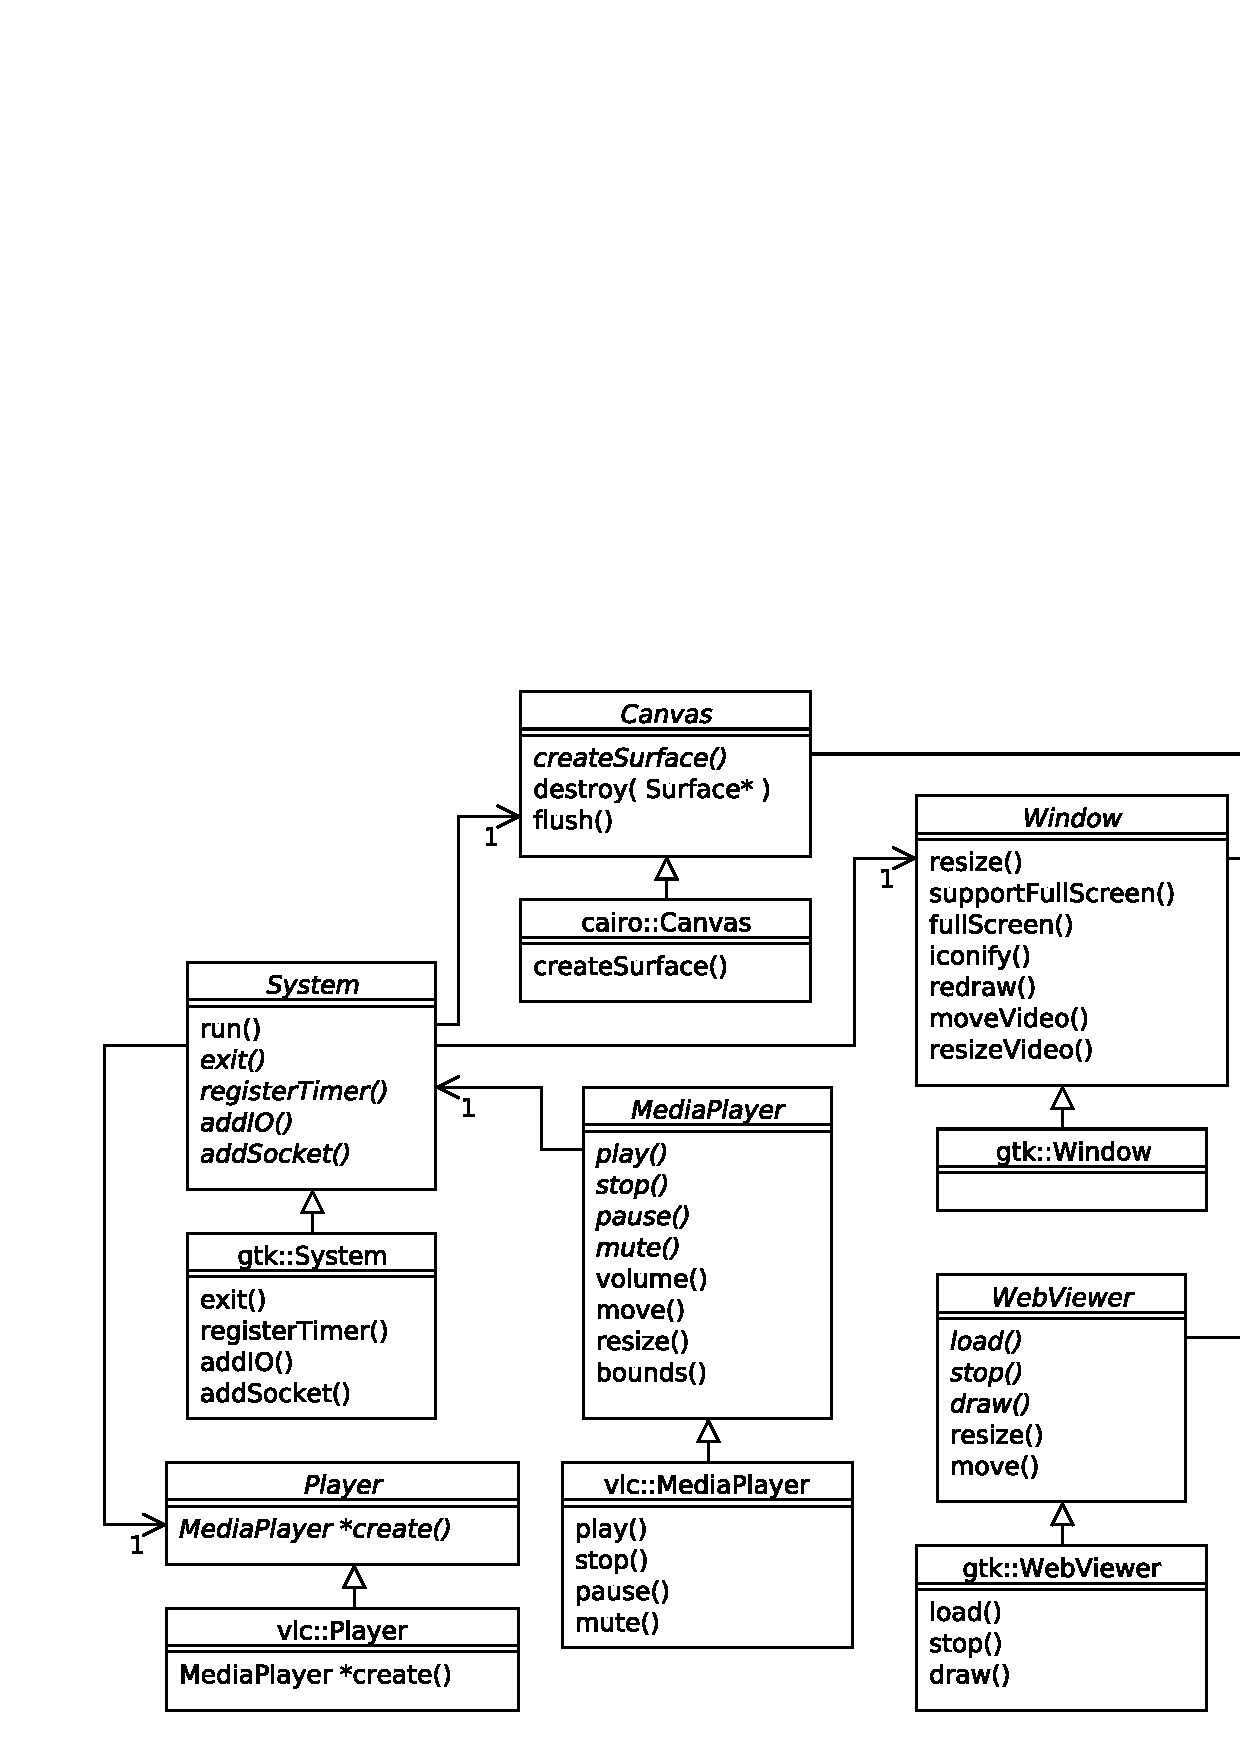
\includegraphics[scale=0.5]{resources/uml-dtv-canvas.jpg}
	\caption{Diagrama de las principales clases de la librería \emph{canvas}.}
\end{figure}

\FloatBarrier
